%% fig_hodgespike.tex   (generated by make_core.py; do not edit by hand)
%% dim Hdg^k(A) for n = 2, 3, 4 (thm:hdgcount): one class eta^k in every degree 0 <= k <= 2n, and the Weil line on top at k = n.
\documentclass[tikz,border=8pt]{standalone}
\usepackage{amsmath,amssymb}
\usetikzlibrary{arrows.meta,calc,decorations.pathreplacing}
%% palette.tex -- shared colour definitions for the figures
\definecolor{PInk}{RGB}{26,32,44}
\definecolor{PBlue}{RGB}{37,82,139}
\definecolor{PTeal}{RGB}{23,127,125}
\definecolor{POchre}{RGB}{193,138,44}
\definecolor{PClay}{RGB}{178,74,58}
\definecolor{PSlate}{RGB}{108,122,137}
\definecolor{PViolet}{RGB}{110,86,150}
\definecolor{WBlue}{RGB}{223,234,246}
\definecolor{WTeal}{RGB}{220,238,236}
\definecolor{WOchre}{RGB}{250,240,218}
\definecolor{WClay}{RGB}{247,229,224}
\definecolor{WSlate}{RGB}{238,241,244}
\definecolor{PMag}{RGB}{158,58,110}
\definecolor{PGrass}{RGB}{62,124,66}
\definecolor{PAmber}{RGB}{214,112,38}
\definecolor{PIndigo}{RGB}{58,64,140}
\definecolor{PRule}{RGB}{176,186,197}

%% shared macros so the standalone figures match the paper
\providecommand{\QQ}{\mathbb{Q}}
\providecommand{\ZZ}{\mathbb{Z}}
\providecommand{\RR}{\mathbb{R}}
\providecommand{\CC}{\mathbb{C}}
\providecommand{\PP}{\mathbb{P}}
\providecommand{\Kx}{K^{\times}}
\providecommand{\HW}{W}
\providecommand{\Nm}{\mathrm{N}}
\providecommand{\Hdg}{\mathrm{Hdg}}
\providecommand{\NS}{\mathrm{NS}}
\providecommand{\cA}{\mathcal{A}}
\providecommand{\cD}{\mathcal{D}}
\providecommand{\cF}{\mathcal{F}}
\providecommand{\cP}{\mathcal{P}}
\providecommand{\cO}{\mathcal{O}}
\providecommand{\cQ}{\mathcal{Q}}
\providecommand{\bbar}[1]{\overline{#1}}
\providecommand{\ch}{\operatorname{ch}}
\providecommand{\End}{\mathrm{End}}
\providecommand{\Ext}{\operatorname{Ext}}
\providecommand{\Supp}{\operatorname{Supp}}

\begin{document}
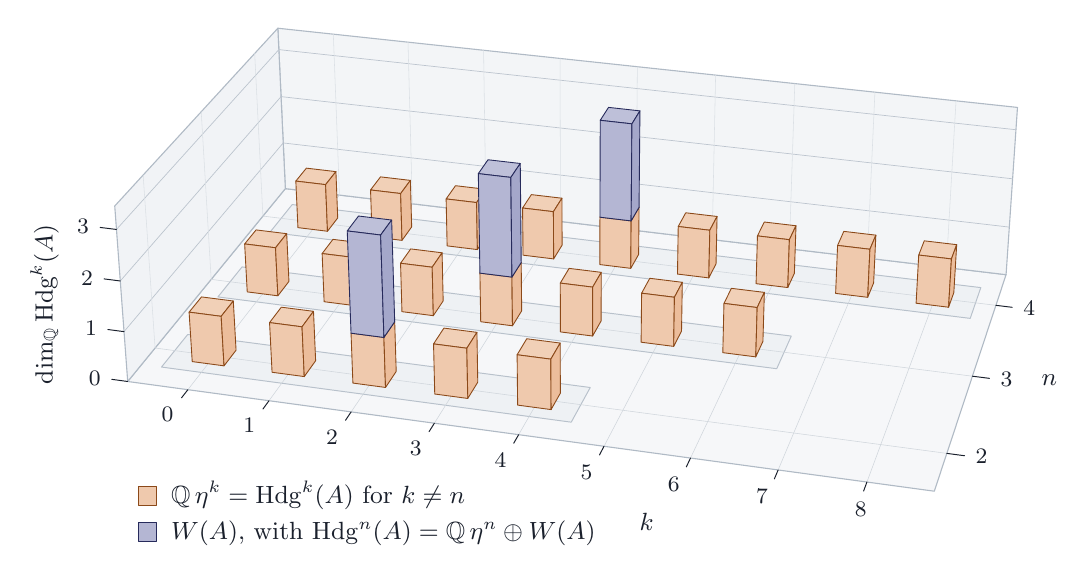
\begin{tikzpicture}[x=1cm,y=1cm,line join=round,line cap=round,
  font=\small,text=PInk,lbl/.style={inner sep=1pt}]
  \path[fill=WSlate!55,draw=PRule,line width=0.40pt] (-5.7547,-1.4506) -- (4.4889,-2.8439) -- (5.4005,-0.0941) -- (-3.7527,0.9990) -- cycle;
  \path[fill=WSlate!70,draw=PRule,line width=0.40pt] (-3.7527,0.9990) -- (5.4005,-0.0941) -- (5.5453,2.0302) -- (-3.8479,3.0359) -- cycle;
  \path[fill=WSlate!85,draw=PRule,line width=0.40pt] (-5.7547,-1.4506) -- (-3.7527,0.9990) -- (-3.8479,3.0359) -- (-5.9194,0.7781) -- cycle;
  \path[fill=WSlate,draw=PRule!90,line width=0.35pt] (-5.3254,-1.2672) -- (-0.1220,-1.9672) -- (0.1196,-1.5269) -- (-4.9927,-0.8536) -- cycle;
  \path[fill=WSlate,draw=PRule!90,line width=0.35pt] (-4.6089,-0.3765) -- (2.4878,-1.2883) -- (2.6728,-0.8738) -- (-4.3025,0.0044) -- cycle;
  \path[fill=WSlate,draw=PRule!90,line width=0.35pt] (-3.9485,0.4444) -- (4.9450,-0.6490) -- (5.0796,-0.2582) -- (-3.6654,0.7963) -- cycle;
  \draw[PRule!85,line width=0.25pt] (-5.8015,-0.8175) -- (-3.7798,1.5789) -- (5.4417,0.5102);
  \draw[PRule!85,line width=0.25pt] (-5.8491,-0.1740) -- (-3.8073,2.1673) -- (5.4835,1.1237);
  \draw[PRule!85,line width=0.25pt] (-5.8974,0.4802) -- (-3.8352,2.7643) -- (5.5260,1.7467);
  \draw[PRule!45,line width=0.2pt] (-3.0654,0.9169) -- (-3.1435,2.9604);
  \draw[PRule!60,line width=0.2pt] (-4.9905,-1.5546) -- (-3.0654,0.9169);
  \draw[PRule!45,line width=0.2pt] (-2.1400,0.8064) -- (-2.1949,2.8589);
  \draw[PRule!60,line width=0.2pt] (-3.9603,-1.6947) -- (-2.1400,0.8064);
  \draw[PRule!45,line width=0.2pt] (-1.2042,0.6947) -- (-1.2352,2.7561);
  \draw[PRule!60,line width=0.2pt] (-2.9169,-1.8366) -- (-1.2042,0.6947);
  \draw[PRule!45,line width=0.2pt] (-0.2577,0.5816) -- (-0.2643,2.6522);
  \draw[PRule!60,line width=0.2pt] (-1.8602,-1.9803) -- (-0.2577,0.5816);
  \draw[PRule!45,line width=0.2pt] (0.6997,0.4673) -- (0.7179,2.5470);
  \draw[PRule!60,line width=0.2pt] (-0.7898,-2.1259) -- (0.6997,0.4673);
  \draw[PRule!45,line width=0.2pt] (1.6680,0.3517) -- (1.7117,2.4406);
  \draw[PRule!60,line width=0.2pt] (0.2944,-2.2734) -- (1.6680,0.3517);
  \draw[PRule!45,line width=0.2pt] (2.6475,0.2347) -- (2.7173,2.3330);
  \draw[PRule!60,line width=0.2pt] (1.3929,-2.4228) -- (2.6475,0.2347);
  \draw[PRule!45,line width=0.2pt] (3.6384,0.1164) -- (3.7349,2.2240);
  \draw[PRule!60,line width=0.2pt] (2.5057,-2.5741) -- (3.6384,0.1164);
  \draw[PRule!45,line width=0.2pt] (4.6409,-0.0033) -- (4.7648,2.1138);
  \draw[PRule!60,line width=0.2pt] (3.6333,-2.7275) -- (4.6409,-0.0033);
  \draw[PRule!60,line width=0.2pt] (-5.4070,-1.0252) -- (4.6481,-2.3635);
  \draw[PRule!45,line width=0.2pt] (-5.4070,-1.0252) -- (-5.5587,1.1712);
  \draw[PRule!60,line width=0.2pt] (-4.6948,-0.1537) -- (4.9731,-1.3833);
  \draw[PRule!45,line width=0.2pt] (-4.6948,-0.1537) -- (-4.8211,1.9752);
  \draw[PRule!60,line width=0.2pt] (-4.0378,0.6502) -- (5.2714,-0.4833);
  \draw[PRule!45,line width=0.2pt] (-4.0378,0.6502) -- (-4.1421,2.7152);
  \path[fill=PAmber!33!white,draw=PAmber!65!black,line width=0.32pt] (-3.6195,1.0945) -- (-3.2413,1.0496) -- (-3.1103,1.2147) -- (-3.4856,1.2589) -- cycle;
  \path[fill=PAmber!38!white,draw=PAmber!65!black,line width=0.32pt] (-3.5929,0.5035) -- (-3.2174,0.4575) -- (-3.2413,1.0496) -- (-3.6195,1.0945) -- cycle;
  \path[fill=PAmber!46!white,draw=PAmber!65!black,line width=0.32pt] (-3.2174,0.4575) -- (-3.0876,0.6264) -- (-3.1103,1.2147) -- (-3.2413,1.0496) -- cycle;
  \path[fill=PAmber!33!white,draw=PAmber!65!black,line width=0.32pt] (-2.6707,0.9819) -- (-2.2881,0.9364) -- (-2.1644,1.1035) -- (-2.5441,1.1481) -- cycle;
  \path[fill=PAmber!38!white,draw=PAmber!65!black,line width=0.32pt] (-2.6509,0.3882) -- (-2.2711,0.3418) -- (-2.2881,0.9364) -- (-2.6707,0.9819) -- cycle;
  \path[fill=PAmber!46!white,draw=PAmber!65!black,line width=0.32pt] (-2.2711,0.3418) -- (-2.1485,0.5126) -- (-2.1644,1.1035) -- (-2.2881,0.9364) -- cycle;
  \path[fill=PAmber!33!white,draw=PAmber!65!black,line width=0.32pt] (-1.7108,0.8679) -- (-1.3238,0.8219) -- (-1.2077,0.9909) -- (-1.5917,1.0361) -- cycle;
  \path[fill=PAmber!38!white,draw=PAmber!65!black,line width=0.32pt] (-1.6981,0.2717) -- (-1.3139,0.2247) -- (-1.3238,0.8219) -- (-1.7108,0.8679) -- cycle;
  \path[fill=PAmber!46!white,draw=PAmber!65!black,line width=0.32pt] (-1.3139,0.2247) -- (-1.1987,0.3975) -- (-1.2077,0.9909) -- (-1.3238,0.8219) -- cycle;
  \path[fill=PAmber!33!white,draw=PAmber!65!black,line width=0.32pt] (-0.7398,0.7526) -- (-0.3482,0.7061) -- (-0.2398,0.8771) -- (-0.6283,0.9228) -- cycle;
  \path[fill=PAmber!38!white,draw=PAmber!65!black,line width=0.32pt] (-0.7342,0.1538) -- (-0.3456,0.1063) -- (-0.3482,0.7061) -- (-0.7398,0.7526) -- cycle;
  \path[fill=PAmber!46!white,draw=PAmber!65!black,line width=0.32pt] (-0.3456,0.1063) -- (-0.2380,0.2811) -- (-0.2398,0.8771) -- (-0.3482,0.7061) -- cycle;
  \path[fill=PAmber!33!white,draw=PAmber!65!black,line width=0.32pt] (1.2368,0.5179) -- (1.6378,0.4703) -- (1.7301,0.6453) -- (1.3325,0.6921) -- cycle;
  \path[fill=PAmber!38!white,draw=PAmber!65!black,line width=0.32pt] (1.2275,-0.0862) -- (1.6253,-0.1348) -- (1.6378,0.4703) -- (1.2368,0.5179) -- cycle;
  \path[fill=PAmber!46!white,draw=PAmber!65!black,line width=0.32pt] (1.6253,-0.1348) -- (1.7171,0.0441) -- (1.7301,0.6453) -- (1.6378,0.4703) -- cycle;
  \path[fill=PAmber!33!white,draw=PAmber!65!black,line width=0.32pt] (0.2427,0.6359) -- (0.6389,0.5889) -- (0.7394,0.7619) -- (0.3464,0.8081) -- cycle;
  \path[fill=PAmber!38!white,draw=PAmber!65!black,line width=0.32pt] (0.2409,0.0345) -- (0.6341,-0.0136) -- (0.6389,0.5889) -- (0.2427,0.6359) -- cycle;
  \path[fill=PAmber!46!white,draw=PAmber!65!black,line width=0.32pt] (0.6341,-0.0136) -- (0.7339,0.1633) -- (0.7394,0.7619) -- (0.6389,0.5889) -- cycle;
  \path[fill=PIndigo!33!white,draw=PIndigo!65!black,line width=0.32pt] (0.2464,1.8665) -- (0.6488,1.8217) -- (0.7507,1.9865) -- (0.3517,2.0305) -- cycle;
  \path[fill=PIndigo!38!white,draw=PIndigo!65!black,line width=0.32pt] (0.2427,0.6359) -- (0.6389,0.5889) -- (0.6488,1.8217) -- (0.2464,1.8665) -- cycle;
  \path[fill=PIndigo!46!white,draw=PIndigo!65!black,line width=0.32pt] (0.6389,0.5889) -- (0.7394,0.7619) -- (0.7507,1.9865) -- (0.6488,1.8217) -- cycle;
  \path[fill=PAmber!33!white,draw=PAmber!65!black,line width=0.32pt] (2.2428,0.3984) -- (2.6485,0.3503) -- (2.7326,0.5274) -- (2.3302,0.5747) -- cycle;
  \path[fill=PAmber!38!white,draw=PAmber!65!black,line width=0.32pt] (2.2257,-0.2083) -- (2.6283,-0.2575) -- (2.6485,0.3503) -- (2.2428,0.3984) -- cycle;
  \path[fill=PAmber!46!white,draw=PAmber!65!black,line width=0.32pt] (2.6283,-0.2575) -- (2.7119,-0.0765) -- (2.7326,0.5274) -- (2.6485,0.3503) -- cycle;
  \path[fill=PAmber!33!white,draw=PAmber!65!black,line width=0.32pt] (-4.2695,0.2964) -- (-3.8773,0.2477) -- (-3.7354,0.4266) -- (-4.1245,0.4745) -- cycle;
  \path[fill=PAmber!38!white,draw=PAmber!65!black,line width=0.32pt] (-4.2368,-0.3126) -- (-3.8476,-0.3623) -- (-3.8773,0.2477) -- (-4.2695,0.2964) -- cycle;
  \path[fill=PAmber!46!white,draw=PAmber!65!black,line width=0.32pt] (-3.8476,-0.3623) -- (-3.7070,-0.1794) -- (-3.7354,0.4266) -- (-3.8773,0.2477) -- cycle;
  \path[fill=PAmber!33!white,draw=PAmber!65!black,line width=0.32pt] (3.2607,0.2776) -- (3.6714,0.2288) -- (3.7469,0.4080) -- (3.3398,0.4560) -- cycle;
  \path[fill=PAmber!38!white,draw=PAmber!65!black,line width=0.32pt] (3.2358,-0.3318) -- (3.6432,-0.3816) -- (3.6714,0.2288) -- (3.2607,0.2776) -- cycle;
  \path[fill=PAmber!46!white,draw=PAmber!65!black,line width=0.32pt] (3.6432,-0.3816) -- (3.7184,-0.1984) -- (3.7469,0.4080) -- (3.6714,0.2288) -- cycle;
  \path[fill=PAmber!33!white,draw=PAmber!65!black,line width=0.32pt] (-3.2855,0.1743) -- (-2.8886,0.1250) -- (-2.7546,0.3061) -- (-3.1483,0.3545) -- cycle;
  \path[fill=PAmber!38!white,draw=PAmber!65!black,line width=0.32pt] (-3.2602,-0.4374) -- (-2.8663,-0.4877) -- (-2.8886,0.1250) -- (-3.2855,0.1743) -- cycle;
  \path[fill=PAmber!46!white,draw=PAmber!65!black,line width=0.32pt] (-2.8663,-0.4877) -- (-2.7335,-0.3026) -- (-2.7546,0.3061) -- (-2.8886,0.1250) -- cycle;
  \path[fill=PAmber!33!white,draw=PAmber!65!black,line width=0.32pt] (4.2910,0.1552) -- (4.7066,0.1059) -- (4.7734,0.2873) -- (4.3614,0.3358) -- cycle;
  \path[fill=PAmber!38!white,draw=PAmber!65!black,line width=0.32pt] (4.2579,-0.4568) -- (4.6702,-0.5073) -- (4.7066,0.1059) -- (4.2910,0.1552) -- cycle;
  \path[fill=PAmber!46!white,draw=PAmber!65!black,line width=0.32pt] (4.6702,-0.5073) -- (4.7369,-0.3219) -- (4.7734,0.2873) -- (4.7066,0.1059) -- cycle;
  \path[fill=PAmber!33!white,draw=PAmber!65!black,line width=0.32pt] (-2.2896,0.0507) -- (-1.8879,0.0009) -- (-1.7620,0.1841) -- (-2.1605,0.2331) -- cycle;
  \path[fill=PAmber!38!white,draw=PAmber!65!black,line width=0.32pt] (-2.2719,-0.5637) -- (-1.8732,-0.6146) -- (-1.8879,0.0009) -- (-2.2896,0.0507) -- cycle;
  \path[fill=PAmber!46!white,draw=PAmber!65!black,line width=0.32pt] (-1.8732,-0.6146) -- (-1.7484,-0.4273) -- (-1.7620,0.1841) -- (-1.8879,0.0009) -- cycle;
  \path[fill=PAmber!33!white,draw=PAmber!65!black,line width=0.32pt] (-0.2612,-0.2010) -- (0.1504,-0.2521) -- (0.2595,-0.0643) -- (-0.1487,-0.0141) -- cycle;
  \path[fill=PAmber!38!white,draw=PAmber!65!black,line width=0.32pt] (-0.2592,-0.8209) -- (0.1493,-0.8731) -- (0.1504,-0.2521) -- (-0.2612,-0.2010) -- cycle;
  \path[fill=PAmber!46!white,draw=PAmber!65!black,line width=0.32pt] (0.1493,-0.8731) -- (0.2575,-0.6812) -- (0.2595,-0.0643) -- (0.1504,-0.2521) -- cycle;
  \path[fill=PAmber!33!white,draw=PAmber!65!black,line width=0.32pt] (-1.2816,-0.0744) -- (-0.8749,-0.1248) -- (-0.7573,0.0607) -- (-1.1607,0.1102) -- cycle;
  \path[fill=PAmber!38!white,draw=PAmber!65!black,line width=0.32pt] (-1.2716,-0.6915) -- (-0.8681,-0.7431) -- (-0.8749,-0.1248) -- (-1.2816,-0.0744) -- cycle;
  \path[fill=PAmber!46!white,draw=PAmber!65!black,line width=0.32pt] (-0.8681,-0.7431) -- (-0.7515,-0.5535) -- (-0.7573,0.0607) -- (-0.8749,-0.1248) -- cycle;
  \path[fill=PIndigo!33!white,draw=PIndigo!65!black,line width=0.32pt] (-1.3020,1.1894) -- (-0.8889,1.1413) -- (-0.7693,1.3182) -- (-1.1790,1.3654) -- cycle;
  \path[fill=PIndigo!38!white,draw=PIndigo!65!black,line width=0.32pt] (-1.2816,-0.0744) -- (-0.8749,-0.1248) -- (-0.8889,1.1413) -- (-1.3020,1.1894) -- cycle;
  \path[fill=PIndigo!46!white,draw=PIndigo!65!black,line width=0.32pt] (-0.8749,-0.1248) -- (-0.7573,0.0607) -- (-0.7693,1.3182) -- (-0.8889,1.1413) -- cycle;
  \path[fill=PAmber!33!white,draw=PAmber!65!black,line width=0.32pt] (0.7717,-0.3292) -- (1.1885,-0.3809) -- (1.2888,-0.1908) -- (0.8756,-0.1400) -- cycle;
  \path[fill=PAmber!38!white,draw=PAmber!65!black,line width=0.32pt] (0.7656,-0.9518) -- (1.1791,-1.0047) -- (1.1885,-0.3809) -- (0.7717,-0.3292) -- cycle;
  \path[fill=PAmber!46!white,draw=PAmber!65!black,line width=0.32pt] (1.1791,-1.0047) -- (1.2787,-0.8105) -- (1.2888,-0.1908) -- (1.1885,-0.3809) -- cycle;
  \path[fill=PAmber!33!white,draw=PAmber!65!black,line width=0.32pt] (1.8175,-0.4589) -- (2.2395,-0.5113) -- (2.3308,-0.3189) -- (1.9125,-0.2674) -- cycle;
  \path[fill=PAmber!38!white,draw=PAmber!65!black,line width=0.32pt] (1.8031,-1.0844) -- (2.2216,-1.1379) -- (2.2395,-0.5113) -- (1.8175,-0.4589) -- cycle;
  \path[fill=PAmber!46!white,draw=PAmber!65!black,line width=0.32pt] (2.2216,-1.1379) -- (2.3125,-0.9413) -- (2.3308,-0.3189) -- (2.2395,-0.5113) -- cycle;
  \path[fill=PAmber!33!white,draw=PAmber!65!black,line width=0.32pt] (-4.9750,-0.5699) -- (-4.5678,-0.6228) -- (-4.4135,-0.4283) -- (-4.8174,-0.3764) -- cycle;
  \path[fill=PAmber!38!white,draw=PAmber!65!black,line width=0.32pt] (-4.9353,-1.1977) -- (-4.5313,-1.2518) -- (-4.5678,-0.6228) -- (-4.9750,-0.5699) -- cycle;
  \path[fill=PAmber!46!white,draw=PAmber!65!black,line width=0.32pt] (-4.5313,-1.2518) -- (-4.3786,-1.0531) -- (-4.4135,-0.4283) -- (-4.5678,-0.6228) -- cycle;
  \path[fill=PAmber!33!white,draw=PAmber!65!black,line width=0.32pt] (-3.9532,-0.7026) -- (-3.5408,-0.7562) -- (-3.3951,-0.5593) -- (-3.8040,-0.5067) -- cycle;
  \path[fill=PAmber!38!white,draw=PAmber!65!black,line width=0.32pt] (-3.9214,-1.3333) -- (-3.5124,-1.3881) -- (-3.5408,-0.7562) -- (-3.9532,-0.7026) -- cycle;
  \path[fill=PAmber!46!white,draw=PAmber!65!black,line width=0.32pt] (-3.5124,-1.3881) -- (-3.3680,-1.1869) -- (-3.3951,-0.5593) -- (-3.5408,-0.7562) -- cycle;
  \path[fill=PAmber!33!white,draw=PAmber!65!black,line width=0.32pt] (-1.8706,-0.9733) -- (-1.4477,-1.0282) -- (-1.3196,-0.8263) -- (-1.7389,-0.7724) -- cycle;
  \path[fill=PAmber!38!white,draw=PAmber!65!black,line width=0.32pt] (-1.8554,-1.6097) -- (-1.4359,-1.6658) -- (-1.4477,-1.0282) -- (-1.8706,-0.9733) -- cycle;
  \path[fill=PAmber!46!white,draw=PAmber!65!black,line width=0.32pt] (-1.4359,-1.6658) -- (-1.3090,-1.4596) -- (-1.3196,-0.8263) -- (-1.4477,-1.0282) -- cycle;
  \path[fill=PAmber!33!white,draw=PAmber!65!black,line width=0.32pt] (-2.9184,-0.8371) -- (-2.5009,-0.8914) -- (-2.3639,-0.6920) -- (-2.7779,-0.6387) -- cycle;
  \path[fill=PAmber!38!white,draw=PAmber!65!black,line width=0.32pt] (-2.8949,-1.4707) -- (-2.4806,-1.5261) -- (-2.5009,-0.8914) -- (-2.9184,-0.8371) -- cycle;
  \path[fill=PAmber!46!white,draw=PAmber!65!black,line width=0.32pt] (-2.4806,-1.5261) -- (-2.3449,-1.3224) -- (-2.3639,-0.6920) -- (-2.5009,-0.8914) -- cycle;
  \path[fill=PIndigo!33!white,draw=PIndigo!65!black,line width=0.32pt] (-2.9667,0.4615) -- (-2.5424,0.4096) -- (-2.4027,0.6000) -- (-2.8235,0.6509) -- cycle;
  \path[fill=PIndigo!38!white,draw=PIndigo!65!black,line width=0.32pt] (-2.9184,-0.8371) -- (-2.5009,-0.8914) -- (-2.5424,0.4096) -- (-2.9667,0.4615) -- cycle;
  \path[fill=PIndigo!46!white,draw=PIndigo!65!black,line width=0.32pt] (-2.5009,-0.8914) -- (-2.3639,-0.6920) -- (-2.4027,0.6000) -- (-2.5424,0.4096) -- cycle;
  \path[fill=PAmber!33!white,draw=PAmber!65!black,line width=0.32pt] (-0.8093,-1.1112) -- (-0.3810,-1.1669) -- (-0.2621,-0.9623) -- (-0.6868,-0.9077) -- cycle;
  \path[fill=PAmber!38!white,draw=PAmber!65!black,line width=0.32pt] (-0.8027,-1.7505) -- (-0.3778,-1.8074) -- (-0.3810,-1.1669) -- (-0.8093,-1.1112) -- cycle;
  \path[fill=PAmber!46!white,draw=PAmber!65!black,line width=0.32pt] (-0.3778,-1.8074) -- (-0.2600,-1.5985) -- (-0.2621,-0.9623) -- (-0.3810,-1.1669) -- cycle;
  \draw[PInk,line width=0.35pt] (-4.9905,-1.5546) -- (-5.0711,-1.6581);
  \draw[PInk,line width=0.35pt] (-3.9603,-1.6947) -- (-4.0366,-1.7995);
  \draw[PInk,line width=0.35pt] (-2.9169,-1.8366) -- (-2.9887,-1.9428);
  \draw[PInk,line width=0.35pt] (-1.8602,-1.9803) -- (-1.9275,-2.0879);
  \draw[PInk,line width=0.35pt] (-0.7898,-2.1259) -- (-0.8524,-2.2349);
  \draw[PInk,line width=0.35pt] (0.2944,-2.2734) -- (0.2367,-2.3837);
  \draw[PInk,line width=0.35pt] (1.3929,-2.4228) -- (1.3401,-2.5346);
  \draw[PInk,line width=0.35pt] (2.5057,-2.5741) -- (2.4580,-2.6874);
  \draw[PInk,line width=0.35pt] (3.6333,-2.7275) -- (3.5909,-2.8423);
  \draw[PInk,line width=0.35pt] (4.6481,-2.3635) -- (4.8732,-2.3935);
  \draw[PInk,line width=0.35pt] (4.9731,-1.3833) -- (5.1890,-1.4107);
  \draw[PInk,line width=0.35pt] (5.2714,-0.4833) -- (5.4788,-0.5085);
  \draw[PInk,line width=0.35pt] (-5.7547,-1.4506) -- (-5.9573,-1.4231);
  \draw[PInk,line width=0.35pt] (-5.8015,-0.8175) -- (-6.0057,-0.7905);
  \draw[PInk,line width=0.35pt] (-5.8491,-0.1740) -- (-6.0548,-0.1476);
  \draw[PInk,line width=0.35pt] (-5.8974,0.4802) -- (-6.1048,0.5059);
  \path[fill=PAmber!38!white,draw=PAmber!65!black,line width=0.32pt] (-5.6247,-3.0206) rectangle (-5.3847,-2.7806);
  \path[fill=PIndigo!38!white,draw=PIndigo!65!black,line width=0.32pt] (-5.6247,-3.4806) rectangle (-5.3847,-3.2406);
  \node[lbl,anchor=east,text=PInk,font=\footnotesize] at (-5.1326,-1.8698) {$0$};
  \node[lbl,anchor=east,text=PInk,font=\footnotesize] at (-4.0954,-2.0132) {$1$};
  \node[lbl,anchor=east,text=PInk,font=\footnotesize] at (-3.0448,-2.1584) {$2$};
  \node[lbl,anchor=east,text=PInk,font=\footnotesize] at (-1.9805,-2.3054) {$3$};
  \node[lbl,anchor=east,text=PInk,font=\footnotesize] at (-0.9022,-2.4543) {$4$};
  \node[lbl,anchor=east,text=PInk,font=\footnotesize] at (0.1903,-2.6051) {$5$};
  \node[lbl,anchor=east,text=PInk,font=\footnotesize] at (1.2974,-2.7578) {$6$};
  \node[lbl,anchor=east,text=PInk,font=\footnotesize] at (2.4192,-2.9124) {$7$};
  \node[lbl,anchor=north,text=PInk,font=\footnotesize] at (3.5562,-2.9361) {$8$};
  \node[lbl,anchor=north,text=PInk] at (0.8366,-3.0789) {$k$};
  \node[lbl,anchor=west,text=PInk,font=\footnotesize] at (4.9723,-2.4067) {$2$};
  \node[lbl,anchor=west,text=PInk,font=\footnotesize] at (5.2882,-1.4233) {$3$};
  \node[lbl,anchor=west,text=PInk,font=\footnotesize] at (5.5781,-0.5206) {$4$};
  \node[lbl,anchor=west,text=PInk] at (5.8090,-1.4307) {$n$};
  \node[lbl,anchor=east,text=PInk,font=\footnotesize] at (-6.0564,-1.4096) {$0$};
  \node[lbl,anchor=east,text=PInk,font=\footnotesize] at (-6.1048,-0.7774) {$1$};
  \node[lbl,anchor=east,text=PInk,font=\footnotesize] at (-6.1540,-0.1349) {$2$};
  \node[lbl,anchor=east,text=PInk,font=\footnotesize] at (-6.2041,0.5183) {$3$};
  \node[lbl,text=PInk,rotate=90] at (-6.8101,-0.4704) {$\dim_{\QQ}\Hdg^{k}(A)$};
  \node[lbl,anchor=west,text=PInk,text height=1.6ex,text depth=0.3ex] at (-5.2447,-2.9006) {$\QQ\,\eta^{k}=\Hdg^{k}(A)$ for $k\neq n$};
  \node[lbl,anchor=west,text=PInk,text height=1.6ex,text depth=0.3ex] at (-5.2447,-3.3606) {$\HW(A)$, with $\Hdg^{n}(A)=\QQ\,\eta^{n}\oplus\HW(A)$};
\end{tikzpicture}
\end{document}
